\chapter{Classifying SLSN using Machine Learning}
\label{Chapter5}
\lhead{Chapter 5. \emph{ML Classification}}

Throughtout this thesis, I worked with an underlying theme of performing SN classifications, focusing particularly on the selection of SLSN. In \cref{Chapter3}, I establised a definition of SLSNe in terms of the parameter space of the spin-down of a Magnetar model, later used to photometrically classify one SLSNe in the SNLS archival data. In this chapter, I start by describing these techniques as applied to the DES data set during the real-time search for SN in seasons two and three. This included both the manual scanning of SNe and combining it with the Magnetar model fitting. While successful in identifying several, later confirmed, candidate SLSNe, a number of misclassifications highlighted a need for a more robust approach.

In recent years the whole field of astronomy entered a new data analysis renaissance, utilising the Big Data tools and Machine Learning techniques to extract more from archival data and prepare for the arrival of new surveys such as Gaia, LSST, SKA that are expected to produce stagering amounts of data. These are not only difficult to handle for astronomers used to working on much smaller data samples but will infact require absolute state-of-the-art facilies and tools to handle and analyse the data streams. Following this revolution, I endevored to apply some of the latest techniques in ML to the problem of SN classification.

To date, there has been a number of SN studies aiming at classifying SN with the help of ML. Here, I am focusing only on the studies classifying the light curves of SNe and not point source classification pipelines such the once used in DES \citep{Goldstein2015} and Suburu \citep{Morii2016}. Amongst a number of similar works \citep{Karpenka2012,Moller2016,Charnock2016} the most thorough and indepth study of ML classification of SNe is presented in \citet{Lochner2016}. In their work, a number of models are used to extract a range of light curve features. They also provide a comparison of a number of Supervised ML algorithms and discuss their merits in terms of SN classification. While thorough in their analysis, their approach is not ready for deployment in a real survey. The training sampled used in their analysis is the SPCC dataset containing a sanitised sample of SNe only. In a survey such as DES we would first have to separate SNe from other types of transients which, when considering ML techniques, can be performed at the same stage as the classification of SNe.

The use of the SPCC dataset, containg only 2000 SNe weighted to match their observed rates, by \citet{Lochner2016} along with all previous ML classification studies of SNe is one of their greatest drawbacks. In this thesis, I aim to provide the first SN classification study utilising a large (tens of thousands objects of each class), artificially generated sample of objects. With the size of the training sample I tackle the common issue with overfitting for the less common subclasses of SNe. Furthermore, by placing the SNe uniformally throughtout the DES observing season and at a wide range of redshifts, I introduce real survey inperfections including objects whoch suffer from season edge effects and low S/N.

One of the greatest differences between all previous studies and this thesis is the family of ML algorithms used. \citet{Lochner2016} used the SALT2 model, in the process commonly refered to in ML as Feature Extraction or Feature Engineering, to extract a set of parameters that describe the light curve. These are then fed into the machine learning algorithm to produce their classifications. In this thesis, I use Convolutional Neural Networks (CNN), an overwelmingly powerful technique which dominates in the world of commercial ML solutions. CNNs, described in detail in \sref{sec:CNN}, use the data directly as they building their feature sets as part of the learning process. The use of a such a complex ML tool is only possible thanks to the size of the training sample and the data augmentation described in \sref{sec:DataAugmentation}.

In this chapter, I describe the process of creating an artificial training sample of SNe for a majority of subclasses, based on the tools developed in \cref{Chapter4}, as well as AGNs and noise spikes which form the majority of transients detected by DES. I then describe the steps taken to apply the survey noise model to the otherwise smooth simulated data before interpolating and ugmenting it with the help of GPR, described in \sref{sec:GP}. Finally, I discuss the use of the CNN framework to provide a photometric classification for all transients detected by DES in the first four years of its operations.

\section{Search for SLSN in DES using a Non-ML}
Before using machine learning to find SLSN I have used the magnetar model in the same way as in \cref{Chapter2}. This did produce some results and resulted in the classification of a few SLSNe in the data, however, we then started finding objects which really did not fit the model at all and sometimes even had a Chi2 of 3000, as in the case of DES15S2nr. Because of this, we knew that we need to try a different approach.

\subsection{Manual scanning of Transients}
text
\subsection{Magnetar Model Fitting}
text

\section{Training sample}
In any ML project, the training sample used to build the classification model is its most import element. Regardless of the algorithm used without the correct samples the model will not be able to accurately label new data and often may fall victim to overfitting. An ideal training set would be large compared to the number of distint classes, containing unambiguesly labelled objects and be indistinguishable from the unlabelled test sample that we wish to classify. In reality, this is difficult to achive and often involves manual scanning and classification of the training sample by the user (e.g the manual scanning of point source detection in DES \citep[][and similar studies]{Goldstein2015}).

In the case of SN light curves building the training sample is very difficult. The data comes from a very wide range of sources as the observations are taken using different telescopes, instruments and filters. The raw numbers of classified SNe are also insufficient with only several thousand objects classified to day [CITE?]. While commonly used, the SPCC dataset does not satisfy the requirement for a CNN training sample as the sample is too small.

In this thesis I, therefore, produce an artificial sample of objects that fit all of our requirements from first principles. For each class of object I determine the parameter space for their respective models that can be used to create a large quantity of perfect light curves in the DES photometric bands with an arbitraty cadence. I then apply the DES cadence and noise model to them, creating simulated survey events that closely resembles the real objects.

\subsection{DES Noise Model} \label{sec:NoiseModel}
The noise model applied to the data in this chapter is based heavily on the routines implemented in the SNANA package \citep{Kessler2009}. SNANA is a very powerful package designed as a tool for a realistic light curve simulations. It was used to simulate the SPCC data set \citep{Kessler2010} as well as generating a sample of SN\,Ia used to determine observational biases in the DES SN cosmology study [WHO DO I CITE; in prep.]. However, due to the design of the package, it is very difficult to implement further models into the code.

In DES, SNANA forms the backbone of the SN analysis and is used to extract the image quality logs from the science and reference frames; including the zero points, PSF and sky backgrounds amongst others. Internally these logs are refered to as the \textsc{SIMLIB} files. I follow the same procedure as implemented in SNANA to determine the uncertainty associated with an observation, given its mjd, observing field, filter and the CCD number. The final flux is then drawn randomly from a Normal distribution centered at the simulated flux, with a variance equal to the estimated uncertainty. To demonstrate the effectiveness of this approach, \fref{fig:IaNoiseComp} shows the comparison between the \textit{r}-band light curve of an example SN\,Ia observed by DES and a simulated light curve denerated based on a SALT2 model (performed using the SNCosmo package \citep{Barbary2014}) fit to the original object. The S/N ratio of the observed and simulated light curves fall close to unity, demonstrating their agreement.

\begin{figure}
  % \includegraphics{/path/to/figure}
  \caption{\textit{Top}: \textit{r}-band light curve of an example SN\,Ia observed by DES and a simulated object created to replicate the original data point. \textit{Bottom}: the ratio of the S/N for the observed and simulated data light curves shown to be in agreement.}
  \label{fig:IaNoiseComp}
\end{figure}

\subsection{SN-Ia}
Amonst the various SN classes simulated in as part of this thesis, SN\,Ia are unquestionably the most well-studied and understood class of objects. Thanks to over two decades of use as cosmological probes, there exists a number of packages able to model and simulate these objects with a high accuracy. Furthermore, the paramater spaces of SN\,Ia as well as peculiar outliries to the class (SN\,Ia-91bg and SN\,Ia-91T) are well understood, gives us a great starting point for our simulations.

While it would be possible to perform our own simulations, starting with any implementation of the SALT2 model (e.g SNANA, SNCosmo or otherwise), and pass these through the DES noise model (\sref{sec:NoiseModel}), I would essentially be replicating the sample of fake SN\,Ia injected into the science images during the live data reduction stages. In DES, these objects are used to estimate the image quality and generate the \textsc{SIMLIB} files making them equivalent to light curve that would be generated through SNANA.

The light curves of SN\,Ia that are injected into the images are generated using the extended SALT2 model as used in \citet{Betoule2014}. The upper redshift range was set as z=1.4 ensuring that the sample is not limited by the simualted redshift. We expect that DES is able to detect SN\,Ia up to redshift z$\sim$1.3. The fake SNe are injected such as to match the rate evolution measured by \citet{Perrett2012}. 50,000 objects have passed the detection criteria and therefore form part of our training sample of SN\,Ia. \fref{fig:IaDist} shows the redshift distribution for the sample.

\begin{figure}
  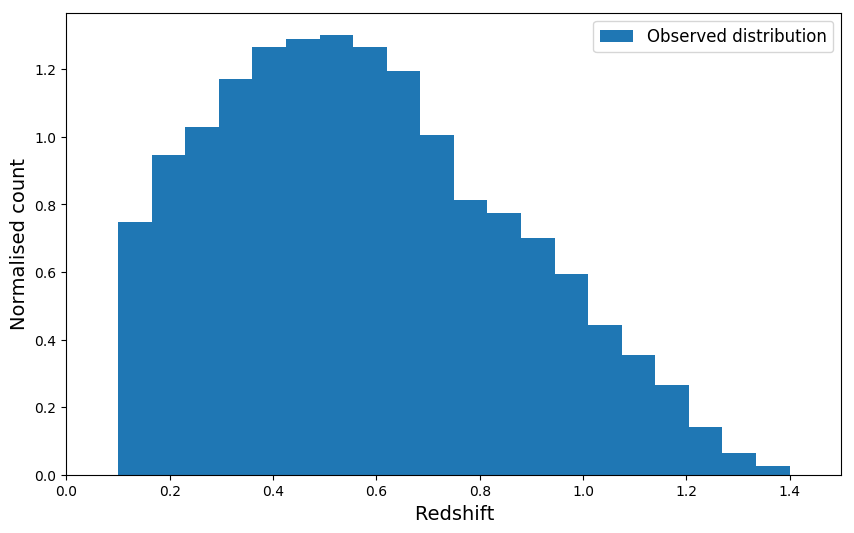
\includegraphics{Figures/Chapter5/SNIa_z_dist.png}
  \caption{The redshift distribution of SN\,Ia that form part of our training sample. }
  \label{fig:IaDist}
\end{figure}

\subsection{CCSN}
While the rate of CCSN is higher than the rate of SN-Ia in the local universe, making the fraction of CCSN to SN-Ia 70\%-30\%, CCSN are a lot fainter objects with an average brightness a tenth of that of SN-Ia. This means that in a survey like DES we can only detect them to the redshift of z$\sim$0.5 instead of the z=1.0 for SN-Ia. The diversity of CCSN is perhaps the greatest amongst our entire training sample ranging between fast, stripped envelope events that can be serious source of contamination for the samples of SN-Ia because of the similarity in their light curves, driven by the powering of Nickel decay in both cases, to long, plotting SN-II which can have a great diversity in their light curve shapes due to the variation in the strength of CSM interactions which powers them.

Many previous attempts were made to make templates of CCSN and use them in packages such as SNANA [CITE EVERYONE]. While from the technical standpoint these were all very good attempts, the biggest drawback suffered by these templates was the scarcity of the data available to make them. Especially in the cases such as SN-Ib, the templates often contain no more than 3 objects. It was therefore pivotal that we expand these templates to the maximum number of objects available in the literature and work on artificially augment the dataset to match the sample size required by Neural Networks.

\subsubsection{Stripped-Envelope SN}
Stripped Envelope SN, namely SN-Ib/c and SN-IIb are a very hot topic in the subject of modelling SN for cosmological purposes. Because their powering mechanism is very similar to that of SN-Ia (e.g. though the decay Ni56 and reprocessing of that radiation in the outter envelope of the ejecta), they often appear extremely similar in light curves causing a potentially large contamination in the sample of photometric SN-Ia that surveys such as DES and LSST may want to use to perform cosmological fitting.

In [CITE CHAPTER 4] I described our approach to creating templates of SN using the CoCo package. While originally written for the PLAsTiCC projects, the code could be trivially extended to DES to produce a large simulation of CCSN. We simulate the CCSN up to z=1.0 as the wide range of possible luminocities does not limit these events from being detected at higher redshift despite the majority of the population expected at z$\sim$0.3. We also assume that the rate of CCSN follows the star formation rate evolution of the universe and anchor the result to the local value found by the SNLS [CITE BAZIN]. \\

\subsubsection{Hydrogen-Rich SN}
Hydrogen-rich SN, or SN-II, are more difficult to define as a class of events than any other type. Their diversity in luminocity can reach over 5 magnitudes and their shapes can vary from SN-Ic like events in case of narrow emission line SN-IIn to long and plateoing SN-IIP events. Nonetheless we must attempt to replicate, to the best of our abilities, the behaviour of these objects for the purpose of our simulations.

We modify the CoCo code [CITE CHAPTER 4] to include XXXXX model [CITE] and found the following templates XXXX [INSERT EVERYTHING THAT BERTIE HAS DONE AND EVERYTHING ELSE THAT I HAVE DONE HERE. IF WE END UP DOING TOO MUCH WORK THIS WILL HAVE TO BECOME ITS OWN SECTION, BUT I DOUBT IT]

\subsection{SLSN}
[CITE : I AM LEAVING THIS SECTION UNTIL I HAVE A MODEL GOOD ENOUGH TO TALK ABOUT, OTHER THAN TOYAH]

\subsection{AGN}
AGN form by far the largest contamination to the survey data. This is partially due to their physical behaviour and partially due to the caveats of the survey design and planning. AGNs often can have a long period of variability leading to the rise and decline in their light curves on scales comparable to SN. In the cases of SLSN, this is particularly troubling as SLSN can be the same duration as a DES observing season making it very possible for an AGN to act as an SLSN impostor if one considers only one season of DES data and not the remainder of the data. Looking at the multi-season light curves it is often very straightforward to identify AGNs though their multi-season variability. A caveat of the survey is that negative "detections" are not considered as detections. This means that if the object was brighter in the SV1 data set, which was used for creating the first set of DES templates than it has been at any point in the first season it would not have been detected until a much later season. Because of this, AGNs have still been misidentified as new transients as late as the last season of DES.

Due to the stochastic nature of AGN, it is now possible to model them in a repetitive way. It is, however, possible to estimate the behaviour of an AGN using a stochastic, random walk model. In this approach, only the basic properties are required such as the mass of the supermassive black hole and the size and orientation of the accretion disk. We use the CODE\_NAME [CITE SEB] to generate 100000 AGN over a period of 10 years of their variability in the DES filters with a daily cadence.

\subsection{Noise}
Visual inspection of the data shows that, while rare, some objects flagged as a real transient according to the DES transient naming criteria \cref{Chapter2} do not appear to be physical in origin. There are two common sources of this: bad subtractions and coincidental noise. Despite the best efforts of the DES transient detection pipeline, some objects (often elongated with negative flux [CITE AND INSERT AN IMAGE]) often pass machine learning with a low score. In some cases (weather dependent or otherwise) this may happen in few consecutive nights leading to a real "transient" flag. Alternatively, a slow-moving object may be detected at the same position in 2 (or 3) consecutive filters at the same position. Usually, this will mean detections in \textit{gri} as \textit{z}-band always has a longer exposure. By itself, this would not result in a "transient" classifications but in combination with bad subtractions of random noise spikes exceeding the 5 sigma detection within 30 days cut can result in a "transient" flag.

To model these objects we can use a very simple approach of inserting a number of sharp spikes in the data, correlated between the filters. This account for the moving objects well. Through testing, we found that to account for bad subtractions the easiest approach is to insert several spikes, with high signal to noise that is correlated both temporally and in flux space.

\subsection{Missing classes}
There are many types of possible transient objects which we have not accounted for here. In some cases we did this because it is unlikely that we would ever detect any (GW counterpart) or because our understanding of them is so limited that we could not provide a comprehensive model for them that could capture the class. This is mostly the case with fast transients [CITE MIIKA] which can appear as having virtually any luminocity and colour and the only connection we have between all of them is their rapid evolution. Believed to be the result of a shock breakout passing though a dense and extended envelope of the star these events are very likely to be connected to the "bumps" often found in SLSN events. We can try to model them as such and see if we can recover such objects [CITE : I REALLY NEED TO TEST THIS, I WOULD HEAVILY BE STEPPING ON MIIKA'S TOES BUT WHO CARES]

\section{Data Augmentation} \label{sec:DataAugmentation}
text
\subsection{Choosing the observing block}
text
\subsection{Choosing the cadence}
text
\subsection{Applying Flux correction to Real Data}
text
\subsection{Applying GPs}
text

\section{Classifications}
text
\subsection{Convolutional Neural Networks}
text
\subsection{Feeding the data}
text
\subsection{SNe vs AGN vs Noise}
text
\subsection{Classifying SNe}
text
\subsection{SLSNe in DES}
